\documentclass[3p,twocolumn]{elsarticle}

\usepackage{graphicx}
\usepackage{color}
\usepackage{url}
\usepackage{float}
\usepackage{listings}   
\usepackage[small,it]{caption}
\usepackage{ifpdf}    
\usepackage{pdfsync}
\usepackage{fancyvrb}
\usepackage{hyperref}

\setlength\parskip{-0.015em}
\setlength\parsep{-0.15em}

\newenvironment{shortlist}{
	\vspace*{-0.85em}
  \begin{itemize}
 \setlength{\itemsep}{-0.3em}
}{
  \end{itemize}
	\vspace*{-0.6em}
}

\DefineShortVerb{\|}
\DefineVerbatimEnvironment{mycode}{Verbatim}
{
  label=Code Example,
  fontsize=\scriptsize,
  frame=single,
% framerule=1pt,
  framesep=0.25em,
  numbers=right,  %numbers=right,
  numbersep=0.5pt,
  gobble=0,
  numberblanklines=false
}

\begin{document}

\title{Understanding Application Level Interoperability: Scaling-Out
  MapReduce From High-Performance Grids to Web-Scale Resources}
\author{Saurabh Sehgal$^?$, Andre Merzky$^{1}$, Shantenu Jha$^{*12}$,  Miklos Erdelyi$^3$ \\
\small{\emph{$^{1}$Center for Computation \& Technology, Louisiana State University, USA}}\\
\small{\emph{$^{2}$Department of Computer Science, Louisiana State University, USA}}\\
\small{\emph{$^{4}$Department of Computer Science and Systems Technology, University of
    Pannonia, Veszprem, Hungary}}\\
\small{\emph{$^{*}$ Contact Author \texttt{sjha@cct.lsu.edu}}}}

\newif\ifdraft
\drafttrue
\ifdraft
\newcommand{\amnote}[1]{ {\textcolor{magenta} { ***AM: #1c }}}
\newcommand{\jhanote}[1]{ {\textcolor{red} { ***SJ: #1 }}}
\newcommand{\miklosnote}[1]{ {\textcolor{blue} { ***ME: #1 }}}
\newcommand{\ssnote}[1]{ {\textcolor{blue} { ***SS: #1 }}}
\else
\newcommand{\amnote}[1]{}
\newcommand{\jhanote}[1]{}
\newcommand{\miklosnote}[1]{}
\newcommand{\ssnote}[1]{}
\fi

\newcommand{\sagamapreduce }{SAGA-MapReduce }
\newcommand{\tc }{ $T_c$ }

\newcommand{\upup}{\vspace*{-0.6em}}
\newcommand{\upp}{\vspace*{-0.6em}}
\newcommand{\up}{\vspace*{-0.3em}}

\newcommand{\T}[1]{\texttt{#1}}
\newcommand{\I}[1]{\textit{#1}}
\newcommand{\B}[1]{\textbf{#1}}

\newcommand{\ssh}[1]{\texttt{ssh}}
\newcommand{\scp}[1]{\texttt{scp}}
\newcommand{\sshfs}[1]{\texttt{sshfs}}
 


%\maketitle
\begin{abstract}
  SAGA is a high-level programming interface which provides the
  ability to develop distributed applications in an infrastructure
  independent way. We discuss how SAGA enables interoperability across
  different distributed infrastructure, but also is to develop a
  version of MapReduce which provides the user with the ability to
  control the relative placement of compute and data.  In this paper,
  we use an application based on SAGA-MapReduce, and demonstrate its
  interoperability across Clouds and Grids at three different levels.
  The primary aim of this paper is to understand different ways in
  which application-level interoperabilty across distributed
  infrastructure can be provided. We achieve this by, (i) developing
  and validating an enhanced verison of MapReduce that scales-out
  across clusters, clouds and HPC resources, (ii) establishing how
  SAGA enables the execution of a scientific application concurrently
  using MapReduce and comparable programming models such as Sphere.
  We also provide a simple performance analysis of \sagamapreduce when
  using multiple, different, heterogeneous infrastructures
  concurrently for the same problem instance.
% However, we do not strive to provide a rigorous performance
%   model, but to provide a proof-of-concept of application-level
%   interoperability and illustrate its importance.
\end{abstract}
\maketitle

\section{Introduction}

% Although Clouds are a nascent infrastructure, there is a ground swell
% in interest to adapt these emerging powerful infrastructure for
% large-scale scientific applications~\cite{montagecloud}. Inevitably,
% and as with any emerging technology, the unified concept of a Cloud --
% if ever there was one, is evolving into different flavours and
% implementations, with distinct underlying system interfaces, semantics
% and infrastructure. For example, the operating environment of Amazon's
% Cloud (EC2) is very different from that of Google's
% Cloud. Specifically for the latter, there already exist multiple
% implementations of Google's Bigtable, such as HyberTable, Cassandra
% and HBase. There is bound to be a continued proliferation of such
% Cloud based infrastructure; this is reminiscent of the plethora of
% Grid middleware distributions.

There are numerous scientific applications that utilize data and
resources distributed over vast heterogeneous infrastructures and
networks with varying speeds and characteristics. However, despite the
drastic differences in hardware capabilities of such distributed
systems, applications usually tend to utilize a single infrastructure
for all of their computational and data processing needs. Since most
distributed frameworks are designed with specific assumptions and
infrastructures in mind, dependence on a single technology in a
heterogeneous environment is not always an optimal choice to gain
maximum runtime performance. For example, the Sector/Sphere data cloud
is exclusively designed to support data-intensive computing on high
speed networks, while other distributed filesystems like GFS/Hadoop
assume limited bandwidth among infrastructure node\cite{}. Thus, for
applications to efficiently utilize heterogeneous environments,
abstractions must be developed for the efficient utilization of and
orchestration across such distinct distributed infrastructure. 

In addition to issues of performance and scale, the transition of
existing distributed programming models and styles, must be as
seamless and as least disruptive as possible.  A fundamental question
at the heart of all these important considerations, is the question of
how scientific applications can be developed so as to utilize as broad
a range of distributed systems as possible, without vendor lock-in,
yet with the flexibility and performance that scientific applications
demand?

Currently, it is unclear what kind of programming models (PM) and
programming systems (PS) will emerge for Clouds; this will
depend, amongst other things, on the kinds of applications that will
come forward to try to utilise Clouds and system-level interfaces that
are exposed by Cloud providers.  Additionally, there are
infrastructure specific features -- technical and policy, that might
influence the design of PM and PS. For example, EC2 -- the archetypal
Cloud System, has a well-defined cost model for data transfer across
{\it its} network. Hence, any PM for Clouds must be cognizant of the
requirement to programmatically control the placement of compute and
data relative to each other -- both statically (pre-run time) and at
run-time.  In general, for most Cloud applications the same
computational task can be priced very differently for possibly the
same performance; conversely, the same computational task can have
very different performance for the same price. It is important for
effective scientific application development on Clouds that, any PM or
PS should not be constrained to a specific infrastructure, i.e.,
should support infrastructure interoperability at the
application-level.

% , we established that the SAGA programming
% system which provides a standard interface, % is an {\it
% %   effective} abstraction that
% can support simple, yet powerful programming models. 

% Work is underway to extend our SAGA based approach in the near
% future to involve tasks with complex and interrelated dependencies.
% Using data-sets of size up to 10GB, and up to 10 workers, we
% provided detailed performance analysis of the SAGA-MapReduce
% implementation, and showed how controlling the distribution of
% computation and the payload-per-worker helped enhance performance. 


% {\it The Case for Interoperabilty:} Interoperability amongst Clouds
% and Grids can be achieved at different levels. For example,
% service-level interoperability amongst Grids has been demonstrated by
% the OGF-GIN group; application-level interoperability (ALI) remains a
% harder goal to achieve.  Clouds provide services at different levels
% (Iaas, PaaS, SaaS); standard interfaces to these different levels do
% not exist.  With an unsettled and rapidly changing Cloud Computing
% landscape, it is unclear if the community is ready for standards-based
% service-level interoperability at the moment.  In addition, t

{\it The Case for Application-level Interoperabilty: } \jhanote{Define
  ALI} ALI arises when, say other than compiling on a different or new
platform, there are no further changes required of the
application. Also, ALI provides automated, generalized and extensible
solutions to use new resources; in some ways, ALI is strong
interoperability, whilst service-level interoperability is weak
interoperability.  The complexity of providing ALI is non-uniform and
depends upon the application under consideration. For example, it is
somewhat easier for simple ``execution unaware'' applications to
utilize heterogeneous multiple distributed environments, than for
applications with multiple distinct and possibly distributed
components. A pre-requisite for ALI is infrastructure independent
programming. Google's MapReduce is tied to Google's file-system;
Hadoop is intrinsically linked to Hadoop file-system (HDFS), as is
Pig.

There is little business motivation for Cloud providers to define,
implement and support new/standard interfaces, there is a case to be
made that applications would benefit from Cloud interoperability.  We
argue that by addressing interoperability at the application-level
this can be easily achieved for both scientific and enterprise
applications.  

In addition there exist a wide range of applications that have
decomposable but heterogeneous computational tasks. It is conceivable,
that some of these tasks are better suited for traditional Grids,
whilst some are better placed in Cloud environments. Montage -- a very
popular Astronomy application provides a prominent example of such an
application.  Additionally, due to different data-compute affinity
requirement amongst the tasks, some workers might be better placed on
a Cloud~\cite{jha_ccpe09}, whilst some may optimally be located on
regular Grids.  Complex dependencies and inter-relationships between
sub-tasks make this often difficult to determine before run-time.

Additionally, with different Clouds providers, fronting different
Economic Models of computing, it is important to be able to utilise
the ``right resource'', in the right way. We briefly discussed how
moving prodigious amounts of data across Cloud networks, as opposed to
moving the compute unit could be expensive.  As current programming
models don't provide explicit support or control for
affinity~\cite{jha_ccpe09}, and in the absence of autonomic
performance models, the end-user is left with performance management,
and with the responsibility of explicitly determining which resource
is optimal. Clearly interoperability between different flavours of
Clouds, and Clouds and Grids is an important pre-requisite.  Finally,
effort directed towards ALI on Clouds/Grids in addition to satisfying
basic curiosity of ``if and how to interoperate'', might also possibly
provide different insight into the programming challenges and
requirements.

% It can be asked if the emphasis on utilising multiple Clouds or Clouds
% and Grids concurrently is premature, given that programming
% models/systems for Clouds are just emerging? In many ways the emphasis
% on interoperability is an appreciation and acknowledgement of an
% application-centric perspective -- that is, as infrastructure changes
% and evolves it is critical to provide seamless transition and
% development pathways for applications and application developers.


% So rather than defend the emphasis on interoperability, we outline
% briefly the motivation/importance for interoperability.  In
% particular we will provide application-level motivation for
% interoperability.

% \jhanote{Mention how we have motivated the need to control
%   relative compute-date placement. This does not really change
%   just because we are using virtualization!}

SAGA or “Simple API for Grid Applications” is a high level API that
provides a simple, standard and uniform interface to the most commonly
required distributed functionality [2]. SAGA can be used to encode
grid applications, tool-kits to manage distributed applications as
well as implement abstractions that support commonly occurring
programming, access and usage patterns. Popular programming
abstractions such as Map-Reduce and All-Pairs have been successfully
implemented with SAGA to showcase its utilization as a flexible
framework to scale-out data-intensive computations on different
flavours of grids and clouds, and attain a high level of
interoperability at the application level. 
 
We focus on MapReduce, which is an application with multiple
homogeneous workers (although the data-load per worker can vary);
however, it is easy to conceive of an application where workers
(tasks) can be heterogeneous, i.e., each worker is different and may
have different data-compute ratios.  In Ref.~\cite{saga_ccgrid09} we
implemented a simple data-parallel programming task (MapReduce) using
SAGA; this involved the concurrent execution of simple,
embarrassingly-parallel data-analysis tasks.  We demonstrated that the
SAGA-based implementation is infrastructure independent whilst still
providing control over the deployment, distribution and run-time
decomposition.  Specifically, we demonstrated that \sagamapreduce is
usable on traditional (Grids) and emerging (Clouds) distributed
infrastructure {\it concurrently and cooperatively towards a solution
  of the same problem instance}.  Our approach was to take
\sagamapreduce and to use the {\it same} implementation of
\sagamapreduce to solve the same instance of the word counting
problem, by using different worker distributions over Clouds and Grid
systems, and thereby also test for interoperability between different
flavours of Clouds as well as between Clouds and Grids.  The primary
focus of this paper is to build upon and use SAGA-based MapReduce as
an exemplar to discuss multiple levels and types of interoperability
that can exist between grids and clouds. This paper is structured as
follows...



% Thanks to the ease of
% developing SAGA “Adaptors”, developers can provide SAGA the interfaces
% to interact with widely different infrastructures simultaneously
% throughout the execution of a single application.


% It is worth mentioning that most
% data-intensive scientific applications fall into this category e.g.,
% high-energy and LIGO data-analysis.  



\section{SAGA}

The SAGA~\cite{saga-core} programming system contains a high level API
that provides a simple, standard and uniform interface for the most
commonly required distributed functionality.  SAGA can be used to
program distributed applications~\cite{saga_escience07, saga_tg08},
tool-kits to manage distributed applications as well as implement
abstractions that support commonly occurring programming, access and
usage patterns.

\begin{figure}[t]
 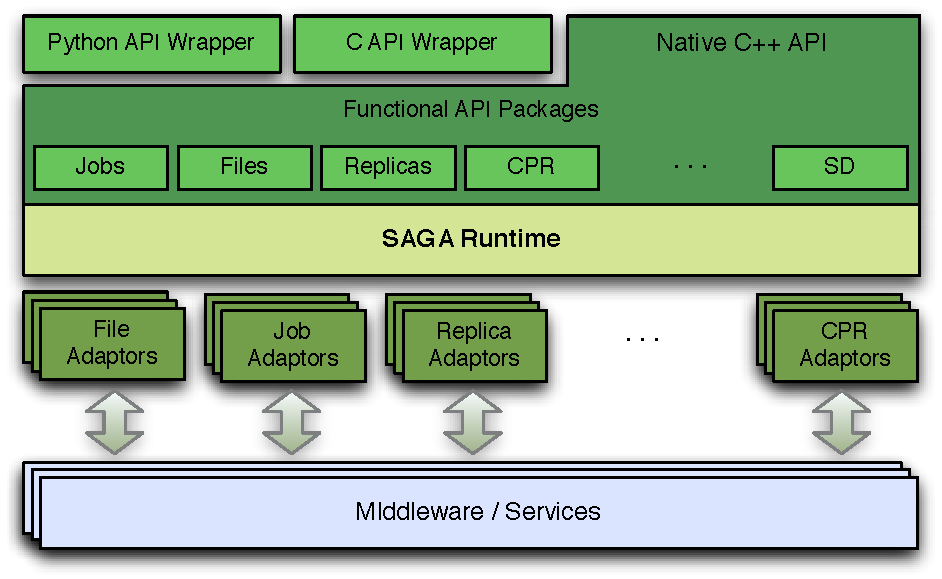
\includegraphics[scale=0.5]{saga-figure02.pdf}
 \caption{The SAGA runtime engine dynamically dispatches high level
          API calls to a variety of middlewares.}
 \label{saga_figure}
\end{figure}

Fig.~\ref{saga_figure} provides an overview of the SAGA programming
system and the main functional areas that SAGA provides a standardized
interface to. Based upon an analysis of more than twenty applications,
the most commonly required functionality involve job submission across
different distributed platforms, support for file access and transfer,
as well as logical file support.  Additionally there is support for
Checkpoint and Recovery (CPR), Service Discovery (SD), and other
areas.  The API is implemented in C++ and Java, with Python supported
as a wrapper. The {\it saga\_core} is the main library, which provides
dynamic support for run-time environment decision making through
loading relevant adaptors. We will not discuss details of SAGA here;
details can be found elsewhere~\cite{saga_url,saga_design}.

\subsection{Interfacing SAGA to Grids and Clouds}

\amnote{TODO: compress, update}

SAGA was originally developed primarily for compute-intensive Grids.
This was a user-driven design decision, i.e., the majority of
applications that motivated the design and formulation of version 1.0
of the API were HPC applications attempting to utilize distributed
resources.  Ref~\cite{saga_ccgrid09} demonstrated that in spite of its
original design constraints, SAGA can be used to develop
data-intensive applications in diverse distributed environments,
including Clouds.  This is in part due to the fact that, at least on
application level, much of the ``distributed functionality'' required
for data-intensive applications remains the same.  In the remainder of
this section, we will describe how, through the creation of a set of
simple context-sensitive {\it adaptors}, the primary functionality of
most applications is supported in an interoperable way.


\subsubsection{Adaptors: Design and Implementation}


\paragraph{SSH adaptors}

The SSH adaptors are based on three different command line tools,
namely \ssh, \scp and \sshfs.  Further, all ssh adaptors rely on the
availability of SSH security credentials for remote operations.  The
SSH context adaptor implements some mechanisms to (a) discover
available key-pairs automatically, and (b) to verify the validity and
usability of the found or otherwise specified credentials.
  
\ssh is used to spawn remote job instances, for which the SSH job
adaptor instantiates a \I{local} \T{saga::job::service} instance, and
submits the respective SSH command lines to it.  The local job adaptor
then takes care of process I/O, detachment, etc.  A significant
drawback of this approach is that several SAGA methods act upon the
local ssh process instead of the remote application instance, which is
far from ideal. Some of these operations can be migrated to the remote
hosts, via separate ssh calls, but that process is complicated due to
the fact that ssh does not report the remote process ID back to the
local job adaptor.  We circumvent this problem by setting a uniquely
identifying environment variable for the remote process, which allows
us to identify the process.

\sshfs is used to access remote files via ssh services.  \sshfs is a
user space file system driver which uses FUSE\ref{fuse}, and is
available for MacOS, Linux, and some other Unix derivatives.  It
enables a remote file system to be mounted into the local namespace,
and transparently forwards all file access operations via ssh to the
remote host.  The ssh file adaptor uses the local job adaptor to call
the sshfs process, to mount the remote filesystem, and then forwards
all file access requests to the local file adaptor, which operates on
the locally mounted file system.  The ssh adaptor thus translates URLs
from the ssh namespace into the local namespace, and back.


\paragraph{AWS adaptors} 

SAGA's AWS (Amazon Web Service) adaptor suite is an interface to
services which implement the cloud web service interfaces as specified
by Amazon~\ref{ec2-url}.  These interfaces are not only used by Amazon
to allow programmatic access to their Cloud infrastructures -- EC2 and
S3, amongst others, but are also used by several other Cloud service
providers, such as Eucalyptus\cite{eucalyptus} and Nimbus.  The AWS
job adaptor is thus able to interface to a variety of Cloud
infrastructures, as long as they adhere to the AWS interfaces.
\amnote{add ref to OCCI, CDMI}

The AWS job adaptor uses the local job adaptor to manage the
invocation of the EC2 command line tools, e.g. to spawn new virtual
machine (VM) instances, to search for existing VM instances, etc.
Once a VM instance is found to be available and ready to accept jobs,
a ssh job service instance for that VM is created, and henceforth
takes care of all job management operations.  The AWS job adaptor is
thus only responsible for VM discovery and management -- the actual
job creation and operations are performed by the ssh job adaptor.  The
security credentials used by the internal ssh job service instance are
derived from the credentials used to create the VM instance.

Note that there is an important semantic difference between 'normal'
(e.g. Grid based) and 'Cloud' job services in SAGA: a normal job
service is assumed to have a lifetime which is completely independent
from the application which accesses that service.  An AWS job service
however points to a potentially volatile resource, or even to a
non-existing resource -- the resource needs then to be created on the
fly.  There are two important implications.  Firstly, the startup time
for a AWS job service is typically much larger than other remote job
service, at least in the case where a VM is created on the fly.  The
second implication is that the \I{end} of the job service lifetime is
usually of no consequence for normal remote job services.  For a
dynamically provisioned VM instance, however, it raises the question
if that instance should be shut down, or if it should automatically
shut down after all remote applications finish, or even if it should
survive for a specific time, or forever.  Ultimately, it is not
possible to control these VM lifetime attributes via the current SAGA
API (by design).  Instead, we allow one of these policies to be chosen
either implicitly (e.g. by using special URLs to request dynamic
provisioning), or explicitly over SAGA config files or environment
variables.  Future SAGA extensions, in particular Resource Discovery
and Resource Reservation extensions, may have a more direct and
explicit notion of resource lifetime management.


\paragraph{Globus Adaptors}

SAGA's globus adaptor suite is amongst its most-utilized adaptors.  As
with ssh, security credentials are expected to be created
out-of-bound, but different credentials can be utilized by pointing
\T{saga::context} instances to them as needed.  Other than the aws and
ssh adaptors, the globus adaptors do not rely on command line tools,
but rather link directly against the respective globus client
libraries: the globus job adaptor is thus a GRAM client, the globus
file adaptor a GridFTP client.  In the experiments, non-Cloud jobs
were started using either GRAM or ssh.  File I/O was performed either
via sshfs, or via a shared Lustre filesystem -- the GridFTP
functionality was not used for experiments in this paper.

\paragraph{Sector-Sphere Adaptors}
Sector and Sphere is a cloud framework specifically designed for
writing applications able to utilize the stream processing
paradigm. Sector is a distributed file system that manages data across
physical compute nodes at the file level, and provides the
infrastructure to manipulate data in the cloud. Sphere, on the other
hand, provides the framework to utilize the stream processing paradigm
for processing the data residing on Sector. The Sphere system is
composed of SPEs or Sphere Processing Units running on the same
physical nodes as the Sector file system.

Applications that utilize the stream processing paradigm define a
single common function (often referred to as a kernel function) that
is applied to segments of a given data set. When the application
invokes Sphere to process data on Sector, the Sphere system retrieves
the stream of data, segments the data and assigns chunks of these
segments to the available SPEs for processing.

Sphere allows the user to encode the kernel function in a dynamically
linked library written using Sphere APIs. The SPEs apply this user
defined function to its assigned segments and write the processing
results back to Sector in files. This stream of output files can be
retrieved by the user from Sector, after the processing is
complete. 

% \ssnote{Maybe add a different section here}
% \ssnote{Add another section here for experiments, or maybe later after
% MapReduce description} 

{\it SAGA adaptor overhead: } We execute a simple experiment to
measure the overhead introduced by submitting Sphere jobs and Sector
file operations through SAGA. A sample Sphere kernel function, wrapped
in a dynamically linked library was used for this purpose. The kernel
function accepts a buffer of text and utilizes the Sphere framework to
hash words into Sphere buckets using the first letter as the key. One
Gigabyte of text data was uploaded to the Sector file system for this
purpose.  Furthermore, traces were implemented in the adaptors to
measure the exact time spent in SAGA processing and translation before
the raw Sphere APIs were called.  As seen in Figure xx, the SAGA
overhead compared to the overall execution time of the application is
negligible. This makes SAGA an excellent platform to compare Sphere
with other distinct programming models.

Thanks to the low overhead of developing SAGA adaptors, we were able
to implement the Sector file adaptor, and the Sphere job adaptor for
applications to utilize the stream processing paradigm through
SAGA. Figure xx and Figure xx give simple examples of how SAGA APIs
can be used to manipulate data in the Sector systems, and how jobs can
be submitted to the Sphere system to process this data.  The
enhancement of SAGA Map Reduce, along with the implementation of the
Sector/Sphere adaptors naturally gives us the opportunity to compare
and study the two distinct programming models.



\section{SAGA-based MapReduce}

% After \sagamapreduce we have also developed real scientific
% applications using SAGA based implementations of patterns for
% data-intensive computing: multiple sequence alignment can be
% orchestrated using the SAGA-All-pairs implementation, and genome
% searching can be implemented using SAGA-MapReduce (see
% Ref.~\cite{saga_ccgrid09}).
% \upup

\subsection{\sagamapreduce Implementation}

Our implementation of \sagamapreduce interleaves the core logic with
explicit instructions on where processes are to be scheduled.  The
advantage of this approach is that our implementation is no longer
bound to run on a system providing the appropriate semantics
originally required by MapReduce, and is portable to a broader range
of generic systems as well.  The drawback is that it is relatively
more complicated to extract performance.% -- for there is a need to add system
% semantic capabilities at some level, and it is inherently slower -- as
% it is difficult to reproduce system-specific optimizations to work
% generically.
The fact that the current implementation is single-threaded
currently is a primary factor for slowdown.  Critically, however, none
of these complexities are transferred to the end-user, and they remain
hidden within the framework. Also many of these are due to the
early-stages of SAGA and incomplete implementation of features, and
not a fundamental limitation of the design or concept of the interface
or programming models that it supports.

% The overall architecture of the SAGA-MapReduce implementation is shown
% in Fig.~\ref{saga-mapreduce_controlflow}. 
This simple interface provides the complete functionality needed by
any MapReduce algorithm, while hiding the more complex functionality,
such as chunking of the input, sorting the intermediate results,
launching and coordinating the workers, etc. as these are implemented
by the framework.  The application consists of two independent
processes, a master and worker processes. The master process is
responsible for:

\begin{itemize}
\item Launching all workers for the map and reduce steps as described
  in a configuration file provided by the user 
\item Coordinating the executed workers, including the chunking of the
  data, assigning the input data to the workers of the map step,
  handling the intermediate data files produced by the map step and
  passing the names of the sorted output files to the workers of the
  reduce step, and collecting the generated outputs from the reduce
  steps and relaunching single worker instances in case of failures,
\end{itemize}

The master process is readily available to the user and needs no
modification for different Map and Reduce functions to execute.  The
worker processes get assigned work either from the map or the reduce
step. The functionality for the different steps have to be provided by
the user, which means the user has to write 2 C++ functions
implementing the required MapReduce algorithm.

Both the master and the worker processes use the SAGA-API as an
abstract interface to the used infrastructure, making the application
portable between different architectures and systems. The worker
processes are launched using the SAGA job package, allowing the jobs
to launch either locally, using globus/GRAM, Amazon Web Services, or
on a Condor pool. The communication between the master and the worker
processes is ensured by using the SAGA advert package, abstracting an
information database in a platform independent way (this can also be
achieved through SAGA-Bigtable adaptors).  The Master process creates
partitions of data (referred to as chunking, analogous to Google's
MapReduce), so the data-set does not have to be on one machine and can
be distributed; this is an important mechanism to avoid limitations in
network bandwidth and data distribution.  These files could then be
recognized by a distributed File-System, such as HDFS.

\subsection{Enhancing SAGA-based Map-Reduce Performance}

%\jhanote{Miklos: This is your section. Please complete/refine/add}

The performance enhancements to the existing \sagamapreduce implementation
are based on two important changes: (i) rearranging the shuffle phase and (ii)
using a serialized binary format instead of plain textual format for intermediate
data storage (also available as an input and output format).  The previous
change means that, instead of having the master merge and then sort the
intermediate data by key before doing the reduce phase, the workers buffer
key/value pairs from the map phase and store them in sorted order
on disk by doing an in-memory sort before writing. Also, since intermediate
key/value pairs from a map worker are already sorted, the reduce workers need
to only merge these pairs coming from different map workers while applying the
user-defined reduce function to the merged intermediate key and value list.
The second important performance enhancement comes from storing intermediate
key/value pairs in a so-called \emph{sequence file format}. This file format
allows storing of serialized key/value objects which can be read and merged
much faster in the reduce phase than textual data because there is no need for
costly parsing.  We used the Google Protocol Buffers library for implementing
serialization \cite{protobuf}.
The processing of input and output key/value pairs is further enhanced by
minimizing unnecessary memory I/O operations using a zero-copy scheme.

\subsection{\sagamapreduce Set-Up \textcolor{red}{Andre}}

\jhanote{compress}
When deploying compute clients on a \I{diverse} set of resources, the
question arises if and how these clients need to be configured to
function properly in the overall application scheme.  \sagamapreduce
compute clients (workers) require two pieces of information to
function: (a) the contact address of the advert service used for
coordinating the clients, and for distributing work items to them; and
(b) a unique worker ID to register with in that advert service, so
that the master can start to assign work items.  Both information are
provided via command line parameters to the worker, at startup time.

The master application requires the following additional information:
i) a set of resources where the workers can execute, ii) location of
the input data, iii) the location of the output data, and iv) the
contact point for the advert service for coordination and
communication.  

In a typical configuration file, for example, three worker instances
could be started; the first could be started via gram and PBS on
qb1.loni.org, second started on a pre-instantiated EC2 image
(instance-id \T{i-760c8c1f}), and finally will be running on a
dynamically deployed EC2 instance (no instance id given).  Note that
the startup times for the individual workers may vary over several
orders of magnitudes, depending on the PBS queue waiting time and VM
startup time.  The mapreduce master will start to utilize workers as
soon as they are able to register themselves, so will not wait until
all workers are available.  That mechanism both minimizes
time-to-solution, and maximizes resilience against worker loss.

The scheme \T{any} acts here as a placeholder for SAGA, so that the
SAGA engine can choose an appropriate adaptor.  The master would
access the file via the default local file adaptor.  The globus
clients may use either the GridFTP or SSH adaptor for remote file
success (but in our experimental setup would also succeed 
using the local file adaptor, as the Lustre FS is mounted on the
cluster nodes), and the EC2 workers would use the ssh file adaptor for
remote access.  Thus, the use of the placeholder scheme frees us from
specifying and maintaining a concise list of remote data access
mechanisms per worker.  Also, it facilitates additional resilience
against service errors and changing configurations, as it leaves it up
to the SAGA engine's adaptor selection mechanism to find a suitable
access mechanism at runtime.
%A parameter not shown in the above configuration example 
A simple parameter can control the number of workers created on each
compute node; as we will see by varying this parameter, the chances
are good that compute and communication times can be interleaved, and
that the overall system utilization can increase (especially in the
absence of precise knowledge of the execution system).
 
% As we have seen above, the globus nodes
% can utilize a variety of mechanisms for accessing the data in
% question.
% include as needed


\section{SAGA-based Applications: Three Types of Interoperabilty}

There are several aspects to interoperability. In this section, we
outline
3 different levels/types of interoperabiltiy...


\subsection{Type I: Application Interoperability on Different
  infrastructure via Adaptors}

A simple form of interoperability is that any application can use any
Clouds systems without changes to the application: the application
simply needs to instantiate a different set of security credentials
for the respective runtime environment. We refer to this as
Cloud-Cloud interoperability. By almost trivial extension, SAGA also
provides Grid-Cloud interoperability, as shown in Fig.~\ref{gramjob}
and ~\ref{vmjob}, where exactly the same interface and functional
calls lead to job submission on Grids or on Clouds. Although
syntactically identical, the semantics of the calls and back-end
management are somewhat different.  As discussed, SAGA provides
interoperability quite trivially thanks to the dynamic loading of
adaptors.  We refer to this as Type I ALI.

hanks to the low overhead of developing adaptors, SAGA has been
deployed on three Cloud Systems -- Amazon,
Eucalyptus~\cite{eucalyptus} (we have a local installation of
Eucalyptus at LSU -- GumboCloud) and Nimbus.

% \begin{verbatim}
% Type I:      Application 
%                   |
%               SAGA-MR
%                   |
%               Different Adaptors


% \end{verbatim}

\subsection{Type II: Application Interopability using programming
  models suited for different infrastructure}

% \begin{verbatim} 
% Type II:     Application 
%                  |
%           Instance-1 Instance-2
%               /        \
%              /          \
%             |            |
%           SAGA-Sphere  SAGA-MapReduce
%             |            |
% Sector-Sphere Clouds    Cluster/Grids
% \end{verbatim}

\subsection{Type III: Application Interoperability using different
  programming models for concurrent execution}


% \begin{verbatim} 
% Type III:   Application Instance
%                 |           
%            SAGA-Sphere and SAGA-MapReduce
%                 |
%  Sector-Sphere Clouds and (Cluster/Grids)
% \end{verbatim}
            

\section{Experiments Demonstrating 3 Types of Interoperabiltiy}

{\it Application - Wordcount: } We implemented two kernel functions to
do a word count on four gigabytes text data.  The first kernel
function is responsible for hashing the words in the data set into
different hashing "buckets". The standard C++ collate hashing function
was used for this purpose. The second kernel function reads each hash
bucket, sorts the words in memory and outputs the final count value of
the words in the data set.  For example, a file containing the words
("bread" "bee" "bee" "honey" ) would be hashed into buckets as -
("bread" "bee" "bee") and ("honey").  The second kernel function would
read these intermediate bucket files, sort the words, and produce the
following result . (.bread 1., .bee 2., .honey 1.).  The Sphere system
is responsible for assigning files for processing, synchronization,
and writing output results back to Sector.


\subsection{Type I: Interoperability via Adaptors}

\subsubsection{Deployment Details}

In order to fully utilize cloud infrastructures for SAGA applications,
the VM instances need to fulfill a couple of prerequisites: the SAGA
libraries and its dependencies need to be deployed, need some external
tools which are used by the SAGA adaptors at runtime -- such as ssh,
SCP, and sshfs.  The latter needs the FUSE kernel module to function
-- so if remote access to the cloud compute node's file system is
wanted, the respective kernel module needs to be installed as well.
There are two basic options to achieve the above, either a customized
VM image which includes all the software that is used, or the
respective packages that are installed after VM instantiation (on the
fly).  Hybrid approaches are possible too.

We support the runtime configuration of VM instances by staging a
preparation script to the VM after its creation, and executing it with
root permissions.  In particular for apt-get linux distribution, the
post-instantiation software deployment is actually fairly painless,
but naturally adds a significant amount of time to the overall VM
startup (which encourages the use of asynchronous operations).
% \footnote{The long VM startup times encourage the use of SAGA's
%   asynchronous operations.}. 
For experiments in this paper, we prepared custom VM images with all
prerequisites pre-installed.  We utilize the preparation script solely
for some fine tuning of parameters: for example, we are able to deploy
custom saga.ini files, or ensure the finalization of service startups
before application deployment\footnote{For example, when starting SAGA
  applications are started before the VM's random generator is
  initialized, our current uuid generator failed to function properly
  -- the preparation script checks for the availability of proper
  uuids, and delays the application deployment as needed.}.

\jhanote{Maybe reduce?} Eucalyptus VM images are basically customized
Xen hypervisor images, as are EC2 VM images.  Customized in this
context means that the images are accompanied by a set of metadata
which tie it to a specific kernel and ramdisk images.  Also, the
images contain specific configurations and startup services which
allow the VM to bootstrap cleanly in the respective Cloud environment,
e.g. to obtain the necessary user credentials, and to perform the
wanted firewall setup etc.  As these systems all use Xen based images,
a conversion of these images for the different cloud systems is in
principle straight-forward.  But sparse documentation and lack of
automatic tools however, make it challenging, at least to the average
end user. Compared to that, the derivation of customized images from
existing images is well documented with well supported tools -- as
long as the target image is to be used on the same Cloud system as the
original one.

% We have also deployed \sagamapreduce to work on Cloud platforms.  It
% is critical to mention that the \sagamapreduce code did not undergo
% any changes whatsoever. 
In executing \sagamapreduce on different Clouds, the change lies in
the run-time system and deployment architecture. For example, when
running \sagamapreduce on EC2, the master process resides on one VM,
while workers reside on different VMs.  Depending on the available
adaptors, Master and Worker can either perform local I/O on a
global/distributed file system, or remote I/O on a remote, non-shared
file system.  % In our current implementation, the VMs hosting the
% master and workers share the same ssh credentials and a shared
% file-system (using sshfs/FUSE). 
Application deployment and configuration (as discussed above) are also
performed via sshfs.  On EC2, we created a custom virtual machine
(VM) image with pre-installed SAGA.  For Eucalyptus, a boot strapping
script equips a standard VM instance with SAGA, and SAGA's
prerequisites (mainly boost).  To us, a mixed approach seemed most
favourable, where the bulk software installation is statically done
via a custom VM image, but software configuration and application
deployment are done dynamically during VM startup.

\subsubsection{Resources used in Experiments}

Simulations were performed on a range of supercomputing resources on
TeraGrid machines, shared TeraGrid-LONI (Louisiana Optical Network
Initiative)~\cite{LONI_web} resources and smaller LONI clusters such
as Eric, Oliver, Louie and Poseidon (512 cores).  We also used
Amazon's EC2 and Nimbus as part of the ScienceCloud at Argonne.

\subsubsection*{Resource I: TeraGrid/LONI Cluster (QB)}

To evaluate the performance of BigJob, several experiments have been
conducted on different LONI resources. The resources used are:
QueenBee (QB), Poseidon and Oliver. For accessing these resources
globus GRAM and an underlying Torque resource manager and Moab
scheduler are used.

\subsubsection*{Resource II: LONI Clusters}
\jhanote{not sure we need this. but just a place-holder for the moment}


\subsubsection*{Resource III: Cloud Environments}
\jhanote{not sure we need this. but just a place-holder for the
  moment; not sure this subsection makes sense. Needs fixing. As does
  the following}

For our experiments we used different Cloud environments: the Nimbus
Science Cloud of the University of Chicago and the Amazon EC2
environment is used. In general, each Cloud has its
characteristics. The Nimbus Cloud is accessed via the WSRF interface,
while for EC2 the Amazon command line client is used. Each Nimbus VM
provides 2 virtual cores and 3.7\,GB memory.  Amazon offeres different
VM types with up to 8 cores. We used the largest VM type (m2.4xlarge)
with 8 cores and 68.4\,GB of memory and the m1.large instance type
with 2 cores and 7.5\,GB, which compares best to the virtual machine
provided by Nimbus.


\subsubsection{Experiments} 

In an earlier paper (Ref~\cite{saga_ccgrid09}), we performed tests to
demonstrate how \sagamapreduce utilizes different infrastructures and
provides control over task-data placement; this led to insight into
performance on ``vanilla'' Grids. The primary aim of this work is to
establish, via well-structured and designed experiments, the fact that
\sagamapreduce has been used to demonstrate Cloud-Cloud
interoperability and Cloud-Grid interoperability. In this paper, we
perform the following experiments:
\begin{enumerate}
\item We compare the performance of \sagamapreduce when exclusively
  running on a Cloud platform to that when on Grids. We vary the
  number of workers (1 to 10) and the data-set sizes varying from 10MB
  to 1GB.
\item For Clouds, we then vary the number of workers per VM, such that
  the ratio is 1:2; we repeat with the ratio at 1:4 -- that is the
  number of workers per VM is 4.
\item We then distribute the same number of workers across two
  different Clouds - EC2 and Eucalyptus.
\item Finally, for a single master, we distribute workers across Grids
  (QueenBee on the TG) and Clouds (EC2 and Eucalyptus) with one job
  per VM.
  % We provide selected performance data.  performance from the two
  % hybrid (EC2-Grid, EC2-Eucalyptus
  % distribution) cases to the pure distributed case.
\end{enumerate}
% Unless mentioned otherwise, we set the number of workers per VM to be
% 1. 
It is worth reiterating, that although we have captured concrete
performance figures, it is not the aim of this work to analyze the
data and provide a performance model. In fact it is difficult to
understand performance implications, as a detailed analysis of the
data and understanding the performance will involve the generation of
``system probes'', as there are differences in the specific Cloud
system implementation and deployment.  For example, in EC2 Clouds % the
% default scenario is probably that the VMs are distributed with respect
% to each other. There
there exists the notion of availability zone, which is really just a
control on which data-center/cluster the VM is placed. In the absence
of explicit mention of the availabilty zone, it is difficult to
determine or assume that the availability zones for multiple,
distributed workers are the same. However, for GumboCloud, it can be
established that the same cluster is used and thus it is fair to
assume that the VMs are local with respect to each other.  Similarly,
without explicit tests, it is often unclear whether data is local or
distributed.  It should also be assumed that for Eucalpytus based
Clouds, data is also locally distributed (i.e.  same cluster with
respect to a VM), whereas for EC2 Clouds this cannot be assumed to be
true for every experiment/test. In a nutshell without adjusting for
different system implementations, it is difficult to rigorously
compare performance figures for different configurations on different
machines. At best we can currently derive trends and qualitative
information.

It takes SAGA about 45s to instantiate a VM on Eucalyptus
\jhanote{Andre is this still true?}  and about 200s on average on EC2.
We find that the size of the image (say 5GB versus 10GB) influences
the time to instantiate an image, but is within image-to-image
instantiation time fluctuation.  Once instantiated, it takes from
1-10s to assign a job to an existing VM on Eucalyptus, or EC2.  The
option to tie the VM lifetime to the \texttt{job\_service} object
lifetime is a configurable option.  It is also a matter of simple
configuration to vary how many jobs (in this case workers) are
assigned to a single VM. The default case is 1 worker per VM; the
ability to vary this number is important -- as details of actual VMs
can differ as well as useful for our experiments.
% it is
% important to be able to vary the number of workers per VM -- as
% details of the VM can differ.

\jhanote{Needs major addition and rewrite. Saurabh and Miklos take a
  first pass please at adding}



\subsubsection{Results and Analysis}


\begin{table}
  \upp
  \footnotesize
  \begin{tabular}{cccccc}
    \hline
    \multicolumn{2}{c}{\#workers}  &  Data size   &  $T_s$  & $T_{sp}$ & $T_s - T_{sp}$\\   
    TG &  AWS &   (MB)  & (sec) & (sec)  & (sec) \\
    \hline
  %  \textcolor{blue}{4} & - & 10  &  8.8 &  6.8 & 2.0 \\
    { {\bf 4}} & - & 10  &  8.8 &  6.8 & 2.0 \\
  %  \textcolor{blue}{6} & - & 10  &  12.4 &  10.2 & 2.2 \\
  %  10 & -  & 100 & 10.4 & 8.86 \\
  %  \textcolor{blue}{10} & - & 10  & 20.8 & 17.3 & 3.5 \\  
    \hline 
    - & 1 & 10 & 4.3 & 2.8 & 1.5 \\
    - & 2 & 10 & 7.8 & 5.3 & 2.5 \\ 
    - & 3 & 10 & 8.7 & 7.7 & 1.0 \\
    - & {\bf 4} & 10 & 13.0 & 10.3 & 2.7 \\
    - & 4 (1) & 10 & 11.3 & 8.6 & 2.7 \\
    - & 4 (2) & 10 & 11.6 & 9.5 & 2.1 \\
    \hline 
    -  & 2  & 100 & 7.9  & 5.3 & 2.6 \\
    -  & {\bf 4}  & 100 & 12.4 & 9.2 & 3.2\\
    -  & 10 & 100 & 29.0 & 25.1 & 3.9 \\
    \hline
    - & {\bf 4 (1)} & 100 & 16.2 & 8.7 & 7.5 \\ 
    - & {\bf 4 (2)} & 100 & 12.3 & 8.5 & 3.8 \\
    - & 6 (3) & 100 & 18.7 & 13.5 & 5.2\\
    - & 8 (1) & 100 & 31.1 & 18.3 & 12.8 \\
    - & 8 (2) & 100 & 27.9 & 19.8 & 8.1\\
    - & 8 (4) & 100 & 27.4 & 19.9 & 7.5\\
    \hline \hline
  \end{tabular}
  \caption{Performance data for different configurations of worker
  placements. The master places the workers on either Clouds or on the
  TeraGrid (TG). The configurations -- separated by horizontal lines,
  are classified as either all workers on the TG or having all workers
  on EC2. For the latter, unless otherwise explicitly indicated by a
  number in parenthesis, every worker is assigned to a unique VM. In
  the final set of rows, the number  in parenthesis indicates the
  number of VMs used. It is interesting to note the significant
  spawning times, and its dependence on the number of VM, which
  typically increase with the number of VMs. $T_{sp}$ (spawn) does not
  include instantiation of the VM.
  \label{stuff-1}}

  
\end{table}

\begin{table}
  \footnotesize
  \begin{tabular}{ccccccc}
    \hline
    \multicolumn{3}{c}{\# workers}  &  Size   &  $T_s$  & $T_{sp}$ & $T_s - T_{sp}$\\   
    TG &  AWS & Eucal. &  (MB)  & (sec) & (sec) & (sec) \\
    \hline
    - & 1 & 1 & 10   & 5.3 & 3.8 & 1.5\\
    - & 2 & 2 & 10   & 10.7 & 8.8 & 1.9 \\
    - & 1 & 1 & 100  & 6.7 & 3.8 & 2.9\\
    - & 2 & 2 & 100  & 10.3 & 7.3 & 3.0\\
    \hline 
    1 & - & 1 & 10   & 4.7 & 3.3 & 1.4\\
    1 & - & 1 & 100  & 6.4 & 3.4 & 3.0\\
    \hline 
    {\bf 2} &   {\bf 2} & - & 10 & 7.4 & 5.9 & 1.5 \\
    3 & 3 & - & 10 & 11.6 & 10.3 & 1.6 \\
    4 & 4 & - & 10 & 13.7 & 11.6 & 2.1 \\
    5 & 5 & - & 10 & 33.2 & 29.4 & 3.8 \\ 
  %\textcolor{blue}{5} & \textcolor{blue}{5} & - & 10 & 33.2 & 29.4 & 3.8 \\ 
    10 & 10 & - & 10 & 32.2 & 28.8 & 2.4 \\
    \hline
     \hline 
  %   1 & 1 & - & 100 & 5.4 & 3.1 & 2.3\\
  %   3 & 3 & - & 100 & 11.1 & 8.7 & 2.4 \\
  \end{tabular}
  \caption{Performance data for different configurations of worker
  placements on TG, Eucalyptus-Cloud and EC2. The first set of data
  establishes Cloud-Cloud interoperability. The second set (rows 5-
  11) shows interoperability between Grids-Clouds (EC2).  The
  experimental conditions and measurements are similar to Table
  1.\label{stuff-2}}
\end{table}



The total time to solution ($T_s$) of a \sagamapreduce job, can be
decomposed as the sum of three primary components -- $t_{over},
t_{comp}$ and $t_{coord}$.  The first term $t_{over}$, is defined as
the time for pre-processing -- which is the time to chunk into fixed
size data units, to distribute them and also to spawn the job. This is
in some ways the overhead of the process (hence the subscript).
Another component of the overhead is the time it takes to instantiate
a VM ($T_{spawn}$).
% It is worth mentioning that currently we instantiate VMs serially as
% opposed to doing this concurrently. This is not a design decision
% but just a quirk, with a trivial fix to eliminate it.
Our performance figures take the net instantiation time into account
and thus normalize for multiple VM instantiation -- whether serial or
concurrent started-up. In fact, for data we report in Table 1 and 2,
the spawning time does not consider instantiation, i.e., the job is
dynamically assigned an existing VM; thus numbers indicate relative
performance and are amenable to direct comparison irrespective of the
number of VMs.  $t_{comp}$ is the time to actually compute the map and
reduce function on a given worker, whilst $t_{coord}$ is the time
taken to assign the payload to a worker, update records and to
possibly move workers to a destination resource; in general,
$t_{coord}$ scales as the number of workers increases.
% In general: \vspace{-1em}
% \begin{eqnarray}
% T_s = t_{over} + t_{comp} + t_{coord} 
% \end{eqnarray}

% We will define $t_{comp} + t_{coord} = T_c = T_s - T_{spawn}$; 
We find that $t_{comp}$ is typically greater than $t_{coord}$, but
when the number of workers gets large, and/or the computational load
per worker small, $t_{coord}$ can dominate (internet-scale
communication) and increase faster than $t_{comp}$ decreases, thus
overall $T_s$ can increase for the same data-set size, even though the
number of independent workers increases.  The number of workers
associated with a VM also influences the performance, as well as the
time to spawn; for example -- as shown by the three lower boldface
entries in Table 1, although 4 identical workers are used depending
upon the number of VMs used, $T_c$ (defined as $T_S - T_{spawn} $) can
be different.  In this case, when 4 workers are spread across 4 VMs
(i.e. default case), $T_c$ is lowest, even though $T_{spawn}$ is the
highest; $T_c$ is highest when all four are clustered onto 1 VM. When
exactly the same experiment is performed using data-set of size 10MB,
it is interesting to observe that $T_c$ is the same for 4 workers
distributed over 1 VM as it is for 4 VMs, whilst when the performance
for the case when  4 workers are spread-over 2 VMs out-perform both (2.1s).
% Interestingly for 100MB and 8 workers -- although the $T_s$ is larger
% than when 4 workers are used, the $T_c$ is lower when 4VMs
% are use

Table 2 shows performance figures when equal number of workers are
spread across two different systems; for the first set of rows,
workers are distributed on EC2 and Eucalyptus. For the next set of
rows, workers are distributed over the TG and Eucalyptus, and in the
final set of rows, workers are distributed between the TG and EC2.
Given the ability to distribute at will, we compare performance for
the following scenarios: (i) when 4 workers are distributed equally
(i.e., 2 each) across a TG machine and on EC2 (1.5s), with the
scenarios when, (ii) all 4 workers are either exclusively on EC2
(2.7s), (iii) or all workers are on the TG machine (2.0s) (see Table
1, boldface entries on the first and fifth line). It is {\it
  interesting} that in this case $T_c$ is lower in the distributed
case than when all workers are executed locally on either EC2 or TG;
we urge that not too much be read into this, as it is just a
coincidence that a {\it sweet spot} was found where on EC2, 4 workers
had a large spawning overhead compared to spawning 2 workers, and an
increase was in place for 2 workers on the TG. Also it is worth
reiterating that for the same configuration there are
experiment-to-experiment fluctuations (typically less than 1s).  The
ability to enhance performance by distributed (heterogeneous)
work-loads across different systems remains a distinct possibility,
however, we believe more systematic studies are required.

% \jhanote{Needs major addition and rewrite. Saurabh and Miklos take a
%   first pass please at adding}

{\it Enhanced SAGA-MR Performance versus Early-version of SAGA-MR}
%\jhanote{Miklos: You have the data for this in the``WordCount
%  Measurement'' tab of
%  \url{http://spreadsheets.google.com/ccc?key=0AvHZsmPSSmBmdHVUMWFuWEpQdFQyak5GeHhQRVJrMlE&hl=en}
%  Please plot and Explain. Related to the earlier sub-section
%  (``Enhancing SAGA-based MapReduce performance) }

\miklosnote{Shantenu: Please correct figure's placement as suitable.}
\jhanote{For the meantime at least, I think this is OK. But we need to 
  describe (in the caption as well) which resources these comparisions were made
  and what the configuration was}

\begin{figure}[htb!]
 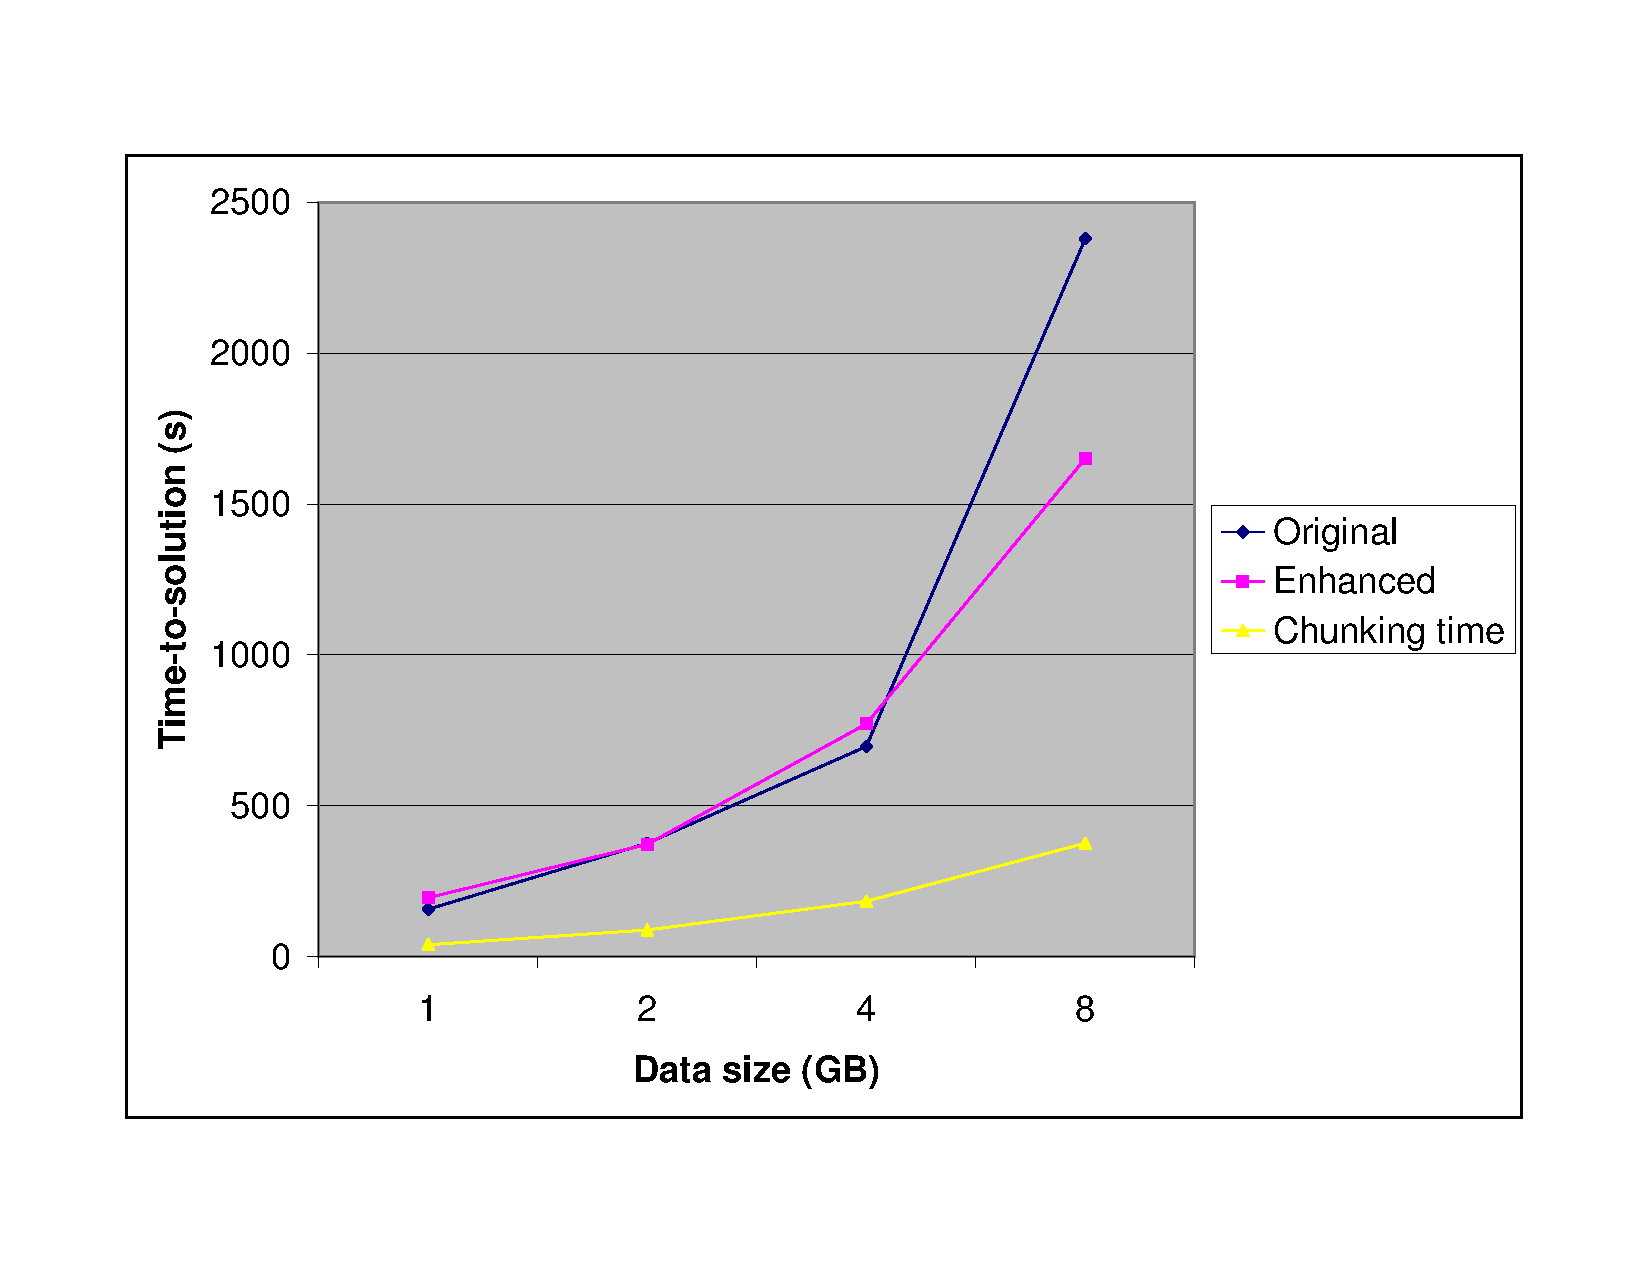
\includegraphics[scale=0.3]{sagamr_original_vs_enhanced.pdf}
 \caption{Comparison of enhanced SAGA-MR performance versus
   early-version of SAGA-MR.}
 \label{sagamr_comparison}
\end{figure}

Since the original \sagamapreduce version chunked the input files and
the enhanced one only creates logical chunks (i.e., no file writing takes
place), it is fair to compare their time-to-solution performance by subtracting
the chunking time from the early-version's job completion time.
Fig.~\ref{sagamr_comparison} shows the performance comparison of the early-version and
enhanced version of \sagamapreduce in such a way.
There were 8 workers spawned via the SAGA SSH job adaptor on 8 physical
machines which exchanged data through a filesystem commonly accessible for all
nodes via NFS. As it can be seen in the figure, the enhancements to \sagamapreduce
start to make a difference when processing at least 4GBs of data.
This can be attributed to the fact that, at this amount of data, the
more efficient shuffle phase implementation which reduces disk I/O and CPU
usage in the reduce phase by doing only a merge outperforms the one with
a merge-sort of all the intermediate output files at once.

\subsection{Type II: Application Performance Using SAGA-based Sphere
  and MapReduce}

{\it Experiment I -- Varying chunk sizes:} Sector maintains and tracks
data in the cloud at the file level. There is no support in Sphere to
control the chunk sizes of files assigned to the Sphere processing
engines. Therefore, to experiment with different chunk sizes, the
files were split manually into smaller chunks before the word count
application was launched. In this set of experiments, we vary the
chunk size from 16MB to 256 MB, while keeping the number of SPEs
constant to 8, and the data size constant to 4 GB. Each SPE is running
on a separate physical node in the cluster. These results are
presented in Figure xx. As evident from the results we collected, a
correlation exists between the chunk sizes and performance of Sphere.
As the chunk sizes increase, the performance deteriorates. Also, we
observe a major decline in performance right after the 64 MB data
point. 

On the other hand, we perform the same set of experiments with
SAGA-MapReduce and observe a completely different trend with respect
to chunk size and performance. SAGA-MapReduce performance increases
with varying chunk sizes, outperforming Sphere at the 256 MB data
point.  \ssnote { Miklos add input here } \jhanote{Saurabh: nice
  write-up. Can you specify the number of workers here. I think it is
  8, but please verify and write}
\ssnote{ Shantenu: I mention the number of workers in the above para.}

{\it Experiment II -- Varying Workers:} We perform two sets of
experiments with SAGA-Sphere running the same word count application.
We keep the chunk size constant at 64 MB, the
data size fixed at 4GB (as previously) but vary the number of
workers in two configurations. In the first configuration, we use Sphere 
on a local data and local compute configuration. In the second configuration, we 
observe how the solution scales to a distributed data and distributed compute
configuration. These results are illustrated in Figure xx and xx.  For
the local-local configuration, we launch Sector and Sphere on a single
physical node. For the distribute-distribute configuration, we launch
Sector and Sphere on one physical node per SPE.  We observe the
maximum peak performance at 6 distributed workers. Sector can be maintain 
file replicas to achieve optimal data distribution between SPEs and minimize
synchronization overhead. For the purpose of our experiments, we
limited Sector to not create any replicas.


SAGA gives us the opportunity to experiment with different programming models very easily. 
As evident from the data plots in Figure xx and Figure yy, certain behavioural 
trends for SAGA-Sphere and SAGA-MapReduce emerge.  In Experiment 1, where we keep the 
number of workers constant and vary the chunk sizes, the trends between 
SAGA-MapReduce and Sphere are opposite. For Sphere, performance deteriorates with 
increasing chunk sizes, while the performance of SAGA-MapReduce increases. This trend 
suggests that SAGA-MapReduce's synchronization overhead to manage smaller 
chunk sizes compared to the speed up achieved through parallelism is much higher. 
This makes SAGA-MapReduce (at least in the case of the word count style applications) a 
better candidate for coarser grained computations. SAGA-Sphere exhibits a 
trend where smaller chunk sizes (a larger amount of files) yield better performance, 
making it suitable for finer grained computations with better data distribution.

In Experiment 2, where we keep the chunk size to a constant of 64 MB, SAGA-Sphere 
exhibits a trend where adding more SPEs has a positive impact on performance. However, 
at the 8 SPEs and 10 SPEs data points, we see a decline in performance, possibly 
due to high synchronization costs between the workers. What is interesting to 
notice are the two data points - 8 SPEs @ 64 MB chunk size in Figure yy 
and 8 SPEs @ 16 MB chunk size in Figure xx. Reducing the chunk size by 25\%, 
thereby providing better data distribution with a larger number of files, we 
see almost a 35\% increase in performance. This further confirms our 
supposition that good data distribution among SPEs is an important factor 
to SAGA-Sphere's performance. 


\subsection{Type  III: Interoperability Concurrency}


\section{Discussion \& Conclusions}

% \subsubsection*{Experience}

% In addition to problems alluded to in earlier footnotes, we mention
% two challenges  faced. We found that the VM images get corrupted, if for
% some reason \sagamapreduce does not terminate properly. Also given
% local firewall and networking policies, we encountered problems in
% initially accessing/addressing the VMs directly.

% We began this paper
% with a discussion of programming systems/model for Clouds, and
% There is a fundamental need for support forfor a programming
% system/model for Clouds.


% however we re-emphasise that the primary strength of SAGA in addition
% to supporting affinity is, i) infrastructure independence, ii) it is
% general-purpose and extensible, iii) provides greater control to the
% end-user if required.

\jhanote{Recap three levels of Application Level Interoperability}

At the lowest level, \sagamapreduce demonstrates how to decouple the
development of applications from the deployment and details of the
run-time environment.  It is critical to reiterate that using this
approach applications remain insulated from any underlying changes in
the infrastructure -- not just Grids and different middleware layers,
but also different systems with very different semantics and
characteristics, whilst being exposed to the important distributed
functionality.  MapReduce has trivial data-parallelism, so in the near
future we will develop applications with non-trivial data-access,
transfer and scheduling characteristics and requirements, and deploy
different parts on different underlying infrastructure guided by
optimal performance.

{\it Programming Models for Clouds: } Ref~\cite{jha_ccpe09} introduced
the notion of {\it affinity} for Clouds to capture the idea of
relative data-compute placement and locality; it is imperative that
any programming model/system be cognizant of the notion of
affinity. We have implemented the first steps in a PM which provides
easy control over relative data-compute placement; a possible next
step would be to extend SAGA to support affinity (data-data,
data-compute).  There exist other emerging programming systems like
Dryad, Sawzall and Pig, which could be used in principle to support
the notion of affinity as well as develop/use MapReduce.  But it is
important to distinguish the infrastructure independence of
\sagamapreduce with the reliance of Google's
MapReduce~\cite{mapreduce-paper} on a number of capabilities of the
underlying system -- mostly related to file operations, but including
system features related to process/data allocation.

We will generalise our approach to most efficiently execute it by
taking into consideration the data-locality, as well as the access
patterns of the execution steps required to complete the work
flow. This analysis is done through developing performance models of
transferring data between frameworks, as well as the distribution of
the computing resources in the environment. Based on this analysis,
the data is placed efficiently, and a subset of nodes and frameworks
maybe chosen to perform the necessary computations. The shuffled data
is also cached for future computations.  e have embarked on the
creation of components that facilitate flexibility in data placement
relative to the computational resource -- that is either data can be
transferred intelligently to match computational workloads or
computational workloads can be placed to match (prevent) data
requirements~\cite{}. More generically, it is worth mentioning that
these approaches can be extend to support certain kinds of {\it
  affinities}.


% A feature worth noting in MapReduce is that the ultimate dataset is
% not on one machine, it is partitioned on multiple machines
% distributed.

% Google use their distributed file system (Google File System) to keep
% track of where each file is located.  Additionally, they coordinate
% this effort with Bigtable.

% {\it Simplicity versus Completeness:} There exist both technical
% reasons and social engineering problems responsible for low uptake of
% Grids. One universally accepted reason is the complexity of Grid
% systems -- the interface, software stack and underlying complexity of
% deploying distributed application. But this is also a consequence of
% the fact that Grid interfaces tend to be ``complete'' or very close
% thereof.  % For example, while certainly not true of all cases, consider
% % the following numbers, which we believe represent the above points
% % well: globus 4.2 provides, in its Java version,
% % approximately 2,000 distinct method calls.  The complete SAGA Core
% % API~\cite{saga-core} provides roughly 200 distinct method calls.
% % The
% % SOAP rendering of the Amazon EC2 cloud interface provides,
% % approximately 30 method calls (and similar for other Amazon Cloud
% % interfaces, such as Eucalyptus~\cite{eucalyptus}).
% The number of
% calls provided by these interfaces is no guarantee of simplicity of
% use, but is a strong indicator of the extent of system semantics
% exposed.  But to a first approximation, (simplicity of) interface
% determines the programming models that can be supported. Thus there is
% the classical trade-off between simplicity and completeness.

%\section{Conclusion and Some Future Directions}

% EC2 and Eucalyptus although distinct systems
% have similar interfaces; we will work towards developing SAGA based
% applications that can use very different infrastructures, e.g.,
% Google's AppEngine, such that \sagamapreduce uses Google's Cloud
% infrastructure.

% Finally, it is worth mentioning that computing in the Clouds for
% this project cost us upwards of \$300 to perform these experiments
% on EC2.

%   somewhat similar; a very different beast is Google's AppEngine.  We
%   will in the near future be working towards providing \sagamapreduce
%   via Google's AppEngine

% {Mention that Amazon and Eucalyptus although distinct are
%   somewhat similar; a very different beast is Google's AppEngine.  We
%   will in the near future be working towards providing \sagamapreduce
%   via Google's AppEngine}


% Patterns capture a dominant and recurring computational mode; by
% providing explicit support for such patterns, end-users and domain
% scientists can reformulate their scientific problems/applications so
% as to use these patterns.  This provides further motivation for
% abstractions at multiple-levels.


%\section{Acknowledgments}
\footnotesize{ {\noindent \bf Acknowledgments: }SJ acknowledges UK EPSRC grant
  number GR/D0766171/1 for supporting SAGA and the e-Science
  Institute, Edinburgh for the research theme, ``Distributed
  Programming Abstractions''.  SJ also acknowledges financial support
  from NSF-Cybertools and NIH-INBRE Grants.  We also acknowledge
  internal resources of the Center for Computation \& Technology (CCT)
  at LSU and computer resources provided by LONI/TeraGrid for
  QueenBee.  We thank Chris Miceli, Michael Miceli, Katerina Stamou \&
  Hartmut Kaiser for their collaborative efforts on early parts of
  this work. We thank Mario Antonioletti and Neil Chue Hong for
  supporting this work through GSoC-2009 (OMII-UK Mentor
  Organisation).}

\bibliographystyle{plain}
\bibliography{saga_data_intensive}
\end{document}

% This work would not have been possible without the efforts and
% support of other members of the SAGA team.  In particular,
% \sagamapreduce was originally written by Chris and Michael Miceli,
% as part of a Google Summer of Code Project, with assistance from
% Hartmut Kaiser. We also thank Hartmut for great support during the
% testing and deployment phases of this project. We are greatful to
% Dmitrii Zagorodnov (UCSB) and Archit Kulshrestha (CyD group, CCT)
% for the support in deployment with Eucalyptus.  KS would like to
% acknowledge the LSU Networking Infrastructure \& Research IT
% Enablement team for their help and support.
